\section{Introduction}
\label{sec:introduction}

\subsection{Anomaly Detection}
\label{subsec:anomaly_detection}

\begin{figure}[t]
    \centering
    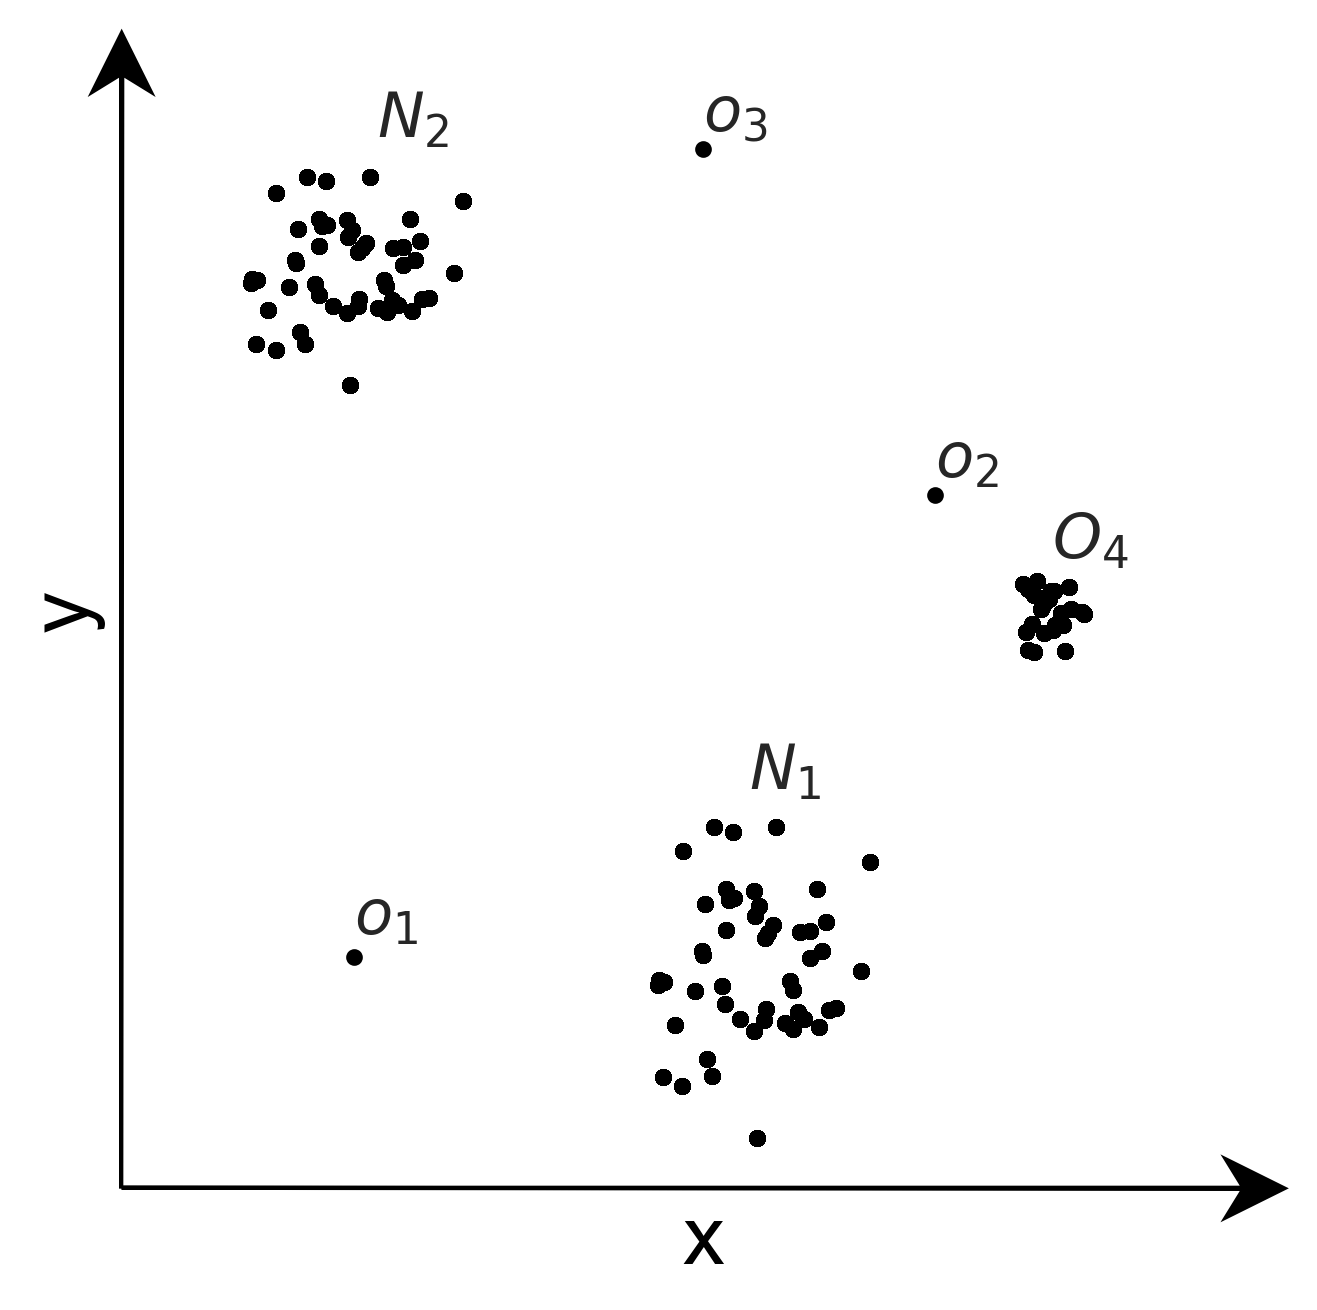
\includegraphics[width=0.6\textwidth]{fig/anomalies.png}
    \caption[Example of Anomalies]{A simple example of a 2D data set containing anomalies, where $N_{1}$ and $N_{2}$ are the `normal' data points and the surrounding points are anomalous.}
    \label{fig:anomalies}
\end{figure}

An anomaly is defined as a data point that does not conform to the expectations of a system, as illustrated in Figure.~\ref{fig:anomalies}. In this example, there are two regions containing normally distributed data, $N_{1}$ and $N_{2}$, where the majority of the data points are concentrated. The surrounding points, $O_{1}$ through to $O_{4}$, are a sufficient distance from the normal data that they are classed as anomalous. Anomaly detection is the process of finding these anomalous data points \cite{huang}. This information can be extremely important and can be applied in a range of ways in order to find out more from a data set. The way in which data is anomalous can also be indicative of what could be the cause, as two different issues could lead to anomalies, and present themselves in different ways. 

The detection of anomalies is crucial both in data cleaning processes, and in the detection of any upcoming issues when monitoring live data \cite{Akouemo2016948}. This has many important real world applications, including those in cyber-security and finance in detecting fraudulent behaviours automatically \cite{618940}. Anomaly detection works under the assumption that a dataset will contain a large number of `normal' points and a few `abnormal' points, taken as the anomalies \cite{Pimentel2014215}. In the scope of this project, anomalies will be produced by unusual behaviour from the motor: caused by issues such as overheating, components beginning to break, or overloading the motor and applying more stress than it can take. 

Anomaly detection has a wide range of real world applications, all of which are crucial when finding issues with equipment in real time or suspicious behaviour in certain data types. Some examples being in credit card fraud detection, medical diagnosis and failure detection in industrial environments. It was first introduced in 1987 for Intrusion Detection Systems (IDS) by Denning for online security, which worked on the assumption that the exploitation of a system's weaknesses would involve abnormal behaviour \cite{1702202}. 

Since this initial application, the use of anomaly detection in cyber-security has become standard, and is crucial for uses such as detecting fraudulent credit card transactions or suspicious online traffic patterns. Before this, one of the first applications of anomaly detection were the Western Electric Rules, which were a set of decision rules that were used to determine `out of control' data (Western Electric Co., \citeyear{statistical_quality_control_handbook_1956}). This was decided by the number of points that were a certain number of standard deviations from the centreline. For example, a single point more than three standard deviations from the centreline or two out of three consecutive points more than two standard deviations away were deemed unstable. These four rules were used to determine when data was beginning to behave in an unpredictable manner. 

Nowadays, anomaly detection has uses in a wide range of fields, including the medical field: Computer Aided Diagnosis (CAD) is used alongside professionals to improve the rates of false positives or undetected anomalies. An anomaly in a mammogram could be an indication of a tumour for example \cite{Sajda2003AMP}. Spacecraft can be monitored using anomaly detection methods to ensure that any failures in equipment are detected early, when the spacecraft is in use and cannot be observed in person \cite{Fujimaki:2005:ADM:2140831.2140938}. Clearly, anomaly detection is a wide ranging field, which has a number of applications in different areas, most of which are extremely important and lead to actionable results.

There are five distinct ways in which anomaly detection can be carried out: probabilistic, distance-based, reconstruction-based, domain-based and information-theoretic based \cite{Pimentel2014215}. The probabilistic approach will estimate the characteristics of a dataset based on the density of points in a `normal' set and compare data to this set to determine which points are anomalous based on the probability of a point being in that position. The distance-based approach assumes that `normal' data will be tightly clustered, and anomalous points will be a distance from these points. Clustering analysis or nearest neighbour analysis is then used to determine whether or not a point is anomalous. Reconstruction-based analysis involves using a training set of data and mapping data using the model that has been created. A large difference between the model and the observed data will result in a high anomaly score, and hence the point will be deemed anomalous. The domain-based approach produces a boundary surrounding the `normal' data, and determines that any point outside of this is anomalous. Finally, using the information-theoretic approach, measures such as entropy are calculated, and it is assumed that anomalous data will significantly change the value of this. A combination of methods will be used to determine where anomalies are found in order to improve the reliability of detecting anomalous points and minimise the chance of false positives.

In our project, anomaly detection has been applied to the vibrations measured on an electric motor whilst running. All electric motors generate vibrations as they move. Analysis of vibration data can be used be used to diagnose the health and general performance of a machine \cite{DelgadoArredondo2017568}. Vibrations in electric motors are caused by forces that are all of a magnetic, mechanical or aerodynamic nature \cite{dorrell_smith_1996}. Various faults and asymmetries have been well identified through vibration signal diagnostics. Typical faults that manifest their signatures in vibration signals include rotor asymmetries, gear faults, unbalanced rotors and faults in the motor bearings. Throughout this project, the vibrations of motors will be monitored, and analysis on this data will allow for the detection of faults. Doing this with live data could mean that faults are detected as they begin, alerting the user and allowing for action before the fault becomes significantly problematic to the system.

Some previous research has been done into vibrational analysis of motors to detect failures. Most examples of this use a distance-based approach or a reconstruction-based approach. In particular, a health index called the Mahalanobis distance has been used as a distance-based approach \cite{Jin20135787} and machine learning has been applied as a reconstruction-based approach \cite{5899067}.

The vibrations from the motor that are being monitored are classed as a continuous signal, as they are taken after equally spaced amounts of time over a given period. This means the data can be defined as time series data, which is simply a series of data points that are taken in chronological order in equally spaced chunks. For scalars this is defined as:

\begin{equation}
    \{x(t_0), x(t_1), ..., x(t_{i-1}), x(t_i), x(t_{i+1}), ...\}~.
\end{equation}

The vibrations of electric motors can be defined as a continuous signal $x(t)$ where $t$ is real-valued. In order to obtain a sample $\{x[t]\}$ one must uniformly sample the signal at discrete points. For a sampling period of $\Delta t$, the obtained sample is defined as,

\begin{equation}
    \{x[t]\} = \{x(0), x(\Delta t), x(2\Delta t), x(3\Delta t),...\}~.
\end{equation}

To recover $x(t)$ from $x[t]$, there must be an appropriate choice for the value of $\Delta t$ in accordance with the Nyquist–Shannon Sampling Theorem. This theorem states that a sampling frequency must be at least twice as high as the highest frequency component of $x(t)$. If not, an aliasing of frequencies will become apparent \cite{Ficker2015}. It is for this reason that 3000 Hz was chosen as the sampling frequency; it is more than double any frequency we expect to measure.

The motivation for this project has been to investigate how motors act when they begin to experience a fault in order to recognise issues in the future. Knowing the way in which a motor behaves when it begins to malfunction could mean motors can be monitored in real time and faults detected as they begin. This could lead to the prevention of some motors malfunctioning completely if the problem is caught early on.

\clearpage
\subsection{Structure of Report}

In \S\ref{sec:methods} we describe the various anomaly detection methods that we have developed and how they have been created and work. We include a discussion about anomaly detection in both the time domain and frequency space. A range of approaches are covered with their positive and negative aspects discussed. Methods that were subsequently rejected have also been mentioned.

In \S\ref{sec:analysis} we examine each motor failure mode that was investigated. The theory behind each failure mode is discussed, as well as the method that we took in order to induce that kind of failure. We then consider the limitations and relative performance of various anomaly detection methods and their various successes at diagnosing particular kinds of motor anomalies.

In \S\ref{sec:conclusion} we discuss the future of anomaly detection, and offer suggestions for future development in the detection of motor anomalies from their vibration signals. The specific methods that we find the most suitable are discussed, as well as the best way to implement the anomaly detection as a whole. We conclude with our final remarks.